\chapter{碳氮库结构}\label{碳氮库结构}
%\addcontentsline{toc}{chapter}{碳氮库结构}

%\begin{碳氮库结构}
CoLM生物地球化学循环模块模拟陆地生态系统碳氮元素储量的动态变化,随着大气$\rm CO_2$浓度升高,
陆地生态系统碳储量的动态模拟反映出陆地生态系统的累积固碳状况。
由于植被和土壤均具有较为稳定的碳氮比属性,氮元素储量的动态模拟,量化了生态系统固碳的氮限制。
碳氮储量在模型中被分为了21个植被碳库、22个植被氮库、7个土壤凋落物碳库和8个土壤凋落物氮库。
运用箱式模型和碳氮平衡方程,碳氮元素在生态系统的传输网络得以刻画,每个碳氮库的动态变化得以模拟。


根据植被次网格结构,植被碳氮库对土壤碳氮库的共享形式存在差异。
LCT次网格结构中,不存在植物类型间土壤无机氮的竞争,
单个植被类型的一套植被碳氮库(21个植被碳库+22个植被氮库)对应一套土壤凋落物碳氮库(7个土壤凋落物碳库+8个土壤凋落物氮库)。
PFT次网格结构中,存在植被类型间的土壤无机氮竞争,多个植被功能型的多套植被氮碳库(n个植被功能型×(21个植被碳库+22个植被氮库))
共享一套土壤凋落物碳氮库(7个土壤凋落物碳库+8个土壤凋落物氮库)。
\section{植被碳氮库结构}\label{植被碳氮库结构}
植被碳库包括叶、细根、活茎、死茎、活粗根和死粗根6个植被营养器官,每个植被营养器官包含组织库、存储库和传输库3类,
因此,每套植被类型有总共18个植被碳库。其中,组织库代表植被营养器官的主要结构组织部分的碳储量,
是植被碳库的主要组成部分;存储碳库和传输碳库分别是长期和短期的非结构碳库,为落叶植被萌发初期提供初始碳,
初始碳供用可以保证植被生长出足够的叶,维持生长季的光合作用。植被氮库除了包含与碳库相对应的18个营养器官氮库之外,
还包含1个再利用氮库,以刻画植被机体在凋落前回收利用氮的生理机能,因此每套植被类型有总共19个植被氮库。
当作物模式打开时,额外增加谷粒器官的组织库、存储库和传输库。因此,总共21个植被碳库和22个植被氮库。
通过对光合作用碳输入的限制,每个植被的碳库和氮库之间具有相对稳定的碳氮比,详见章节 \ref{植被土壤的氮竞争} 植被土壤的氮竞争。

植被碳库之间或植被氮库之间存在复杂的元素循环网络,见图 \ref{fig:CoLM植被碳氮循环网络示意图}。
植被从光合作用中得到碳,并分配到不同器官。存储库、传输库和组织库的元素循环、
叶和活根的胁迫凋落和季节凋落将在章节 \ref{植被物候过程的耦合预报方案} 植被的物候过程中介绍。
活茎和活粗根每年将有固定比例的碳分别转至死茎和死粗根的碳库中。
死茎和死粗根的周转仅存在于植被的自然死亡或火灾中。
{
\begin{figure}[]
\centering
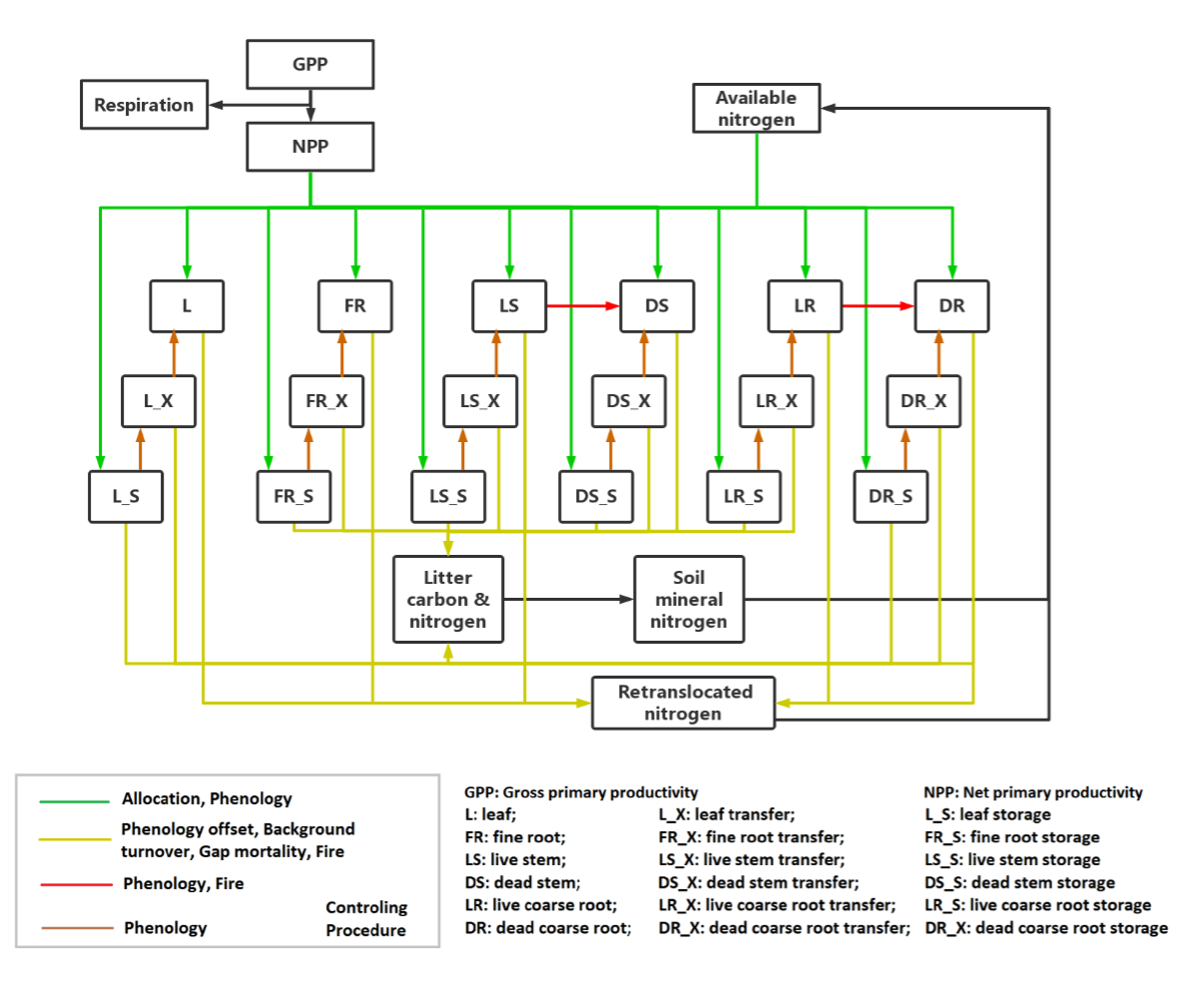
\includegraphics{Figures/碳氮库结构/CoLM植被碳氮循环网络示意图.png}
\caption{CoLM植被碳氮循环网络示意图 \citep{lu2020full}。}
\label{fig:CoLM植被碳氮循环网络示意图}
\end{figure}
}

\section{土壤凋落物碳氮库结构}\label{土壤凋落物碳氮库结构}
土壤凋落物的碳储存同样动态模拟,被按照成分和周转时间的长短进行分类,土壤凋落物碳氮库均具有垂直分层结构的刻画。
\subsection{碳氮库分类}\label{碳氮库分类}
土壤凋落物的碳储分为7个有机碳库:代谢凋落物、纤维素凋落物、木质素凋落物、粗木质残体、快速土壤周转库、
慢速土壤周转库和惰性土壤周转库。凋落物和快速土壤周转库的周转时间都在几个月到几年之间,粗木质残体、
慢速土壤周转库和惰性土壤周转库的周转时间范围分布可以从几年到上千年,表现出极大的土壤异质性。
氮存储除了以上7个有机库外,还包括1个无机氮库。由于植被根系吸收只能利用无机氮,无机氮库是连接土壤和植被的枢纽,
土壤和植被对无机氮的竞争将在章节 \ref{植被土壤的氮竞争} 中介绍。


通过从植被库中获取凋落物,地下元素循环从凋落物到土壤存在较为复杂的元素循环网络,
见图 \ref{fig:CoLM土壤凋落物碳氮循环网络示意图}。土壤碳库和土壤氮库之间在循环过程中保持相对稳定的碳氮比,凋落物的碳氮比大于土壤库的碳氮比,
因此缺氮会造成凋落物的分解速率下降,详见章节 \ref{土壤分解的氮限制} 氮限制因子。
{
\begin{figure}[]
\centering
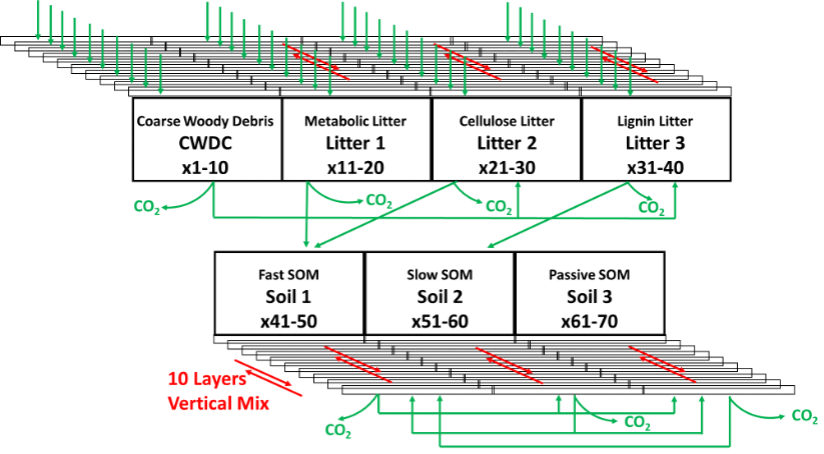
\includegraphics{Figures/碳氮库结构/CoLM土壤凋落物碳氮循环网络示意图.png}
\caption{CoLM土壤凋落物碳氮循环网络示意图 \citep{huang2018matrix}。  }
\label{fig:CoLM土壤凋落物碳氮循环网络示意图}
\end{figure}
}
\subsection{垂直分层结构}\label{垂直分层结构}
由于土壤水热条件的垂直差异,土壤碳氮存储垂直分布模拟也极其重要,且与土壤水热条件的垂直分布特点联系紧密。
CoLM模拟土壤和凋落物的碳氮库垂直结构,与土壤水热模拟保持一致,土壤和凋落物的碳氮库垂直方向上也分为10层。
每层土壤和凋落物分别具有不同的输入(叶片和根系的凋落输入)和输出(分解呼吸)。
同时,除了粗木质残体以外的6个有机库均存在碳氮有机物的垂直扩散混合过程,体现了微生物的作用,详见章节 \ref{土壤凋落物的垂直传输} 土壤凋落物的垂直传输过程。
